
\subsection{Across farm instances}

Every number reported above comes from one farm. Because field areas, soil
drainage, microclimate offsets and parent thermal-time requirements are all
drawn at random, a single instance can be unrepresentative, so we repeated
the comparison on 10 independently generated farms.

It is. Table~\ref{tab:farms} gives the per-farm result and
Fig.~\ref{fig:farms}(a) orders them. The gain from adaptivity averages
1.91\% across farms (SD 1.49, range -0.56\% to +3.94\%),
positive on 9 of 10 farms and individually significant on only
5. Treating the farm as the unit of analysis, the mean gain differs
from zero ($p = 0.003$, Wilcoxon $p = 0.006$), so the effect is real.

Its size, however, is roughly half what the single-instance study reported.
The farm used there ranks 2 of 10, and the 3.9\%
measured on it sits near the top of the distribution. On the best-performing
farm the gain is slightly negative. We report this because it is the kind of
error that a single-instance design cannot reveal, and because the corrected
value strengthens rather than weakens the paper's conclusion: at
1.91\%, adaptive replanning is further below the threshold at which the
irrigation literature judged it not worth its cost.

A second pattern explains much of the spread. The gain is strongly
anti-correlated with how well the farm's static plan already performs
($r = -0.75$, $p = 0.013$; Spearman $\rho = -0.77$),
Fig.~\ref{fig:farms}(b). A farm whose fields and parent lines happen to line
up well needs no adaptation, because a good fixed plan already reaches the
synchrony optimum; adaptivity recovers losses rather than creating gains.
This is directly usable: a producer can estimate in advance whether adaptive
scheduling is worth installing by checking how close a static plan already
gets.

\begin{table}[t]
\caption{Adaptivity gain by farm instance ($\lambda = 1$)}
\label{tab:farms}
\centering\footnotesize
\setlength{\tabcolsep}{4pt}
\begin{tabular}{rrrrrl}
\toprule
Farm & S3 (t) & S4 (t) & $\Delta$ (t) & $\Delta$ (\%) & Sig. \\
\midrule
1 & 102.6 & 104.1 & +1.52 & +1.48 & $p = 0.172$ \\
2 & 107.5 & 108.8 & +1.28 & +1.19 & $p = 0.253$ \\
3 & 98.8 & 100.3 & +1.48 & +1.50 & $p = 0.179$ \\
4 & 110.7 & 110.1 & -0.62 & -0.56 & $p = 0.684$ \\
5 & 85.7 & 88.6 & +2.98 & +3.47 & $p = 0.003$ \\
6 & 105.9 & 107.7 & +1.81 & +1.71 & $p = 0.029$ \\
7 & 101.6 & 105.4 & +3.83 & +3.77 & $p = 0.002$ \\
8 & 93.4 & 95.5 & +2.15 & +2.30 & $p = 0.032$ \\
9 & 88.4 & 91.9 & +3.48 & +3.94 & $p = 0.001$ \\
10 & 101.7 & 102.0 & +0.26 & +0.26 & $p = 0.749$ \\
\midrule
Mean & & & +1.82 & 1.91 & $p = 0.003$ \\
\bottomrule
\end{tabular}
\end{table}

\begin{figure}[t]
\centering
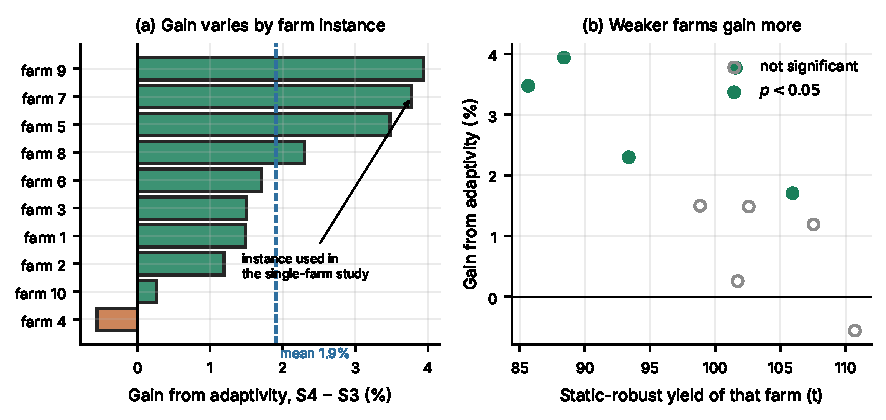
\includegraphics[width=\columnwidth]{../figs/fig5_multifarm.pdf}
\caption{(a) Adaptivity gain on each of 10 independently generated
farms; the outlined bar is the instance used for the single-farm analysis.
(b) The gain is largest on farms whose static plan performs worst.}
\label{fig:farms}
\end{figure}

\subsection{Sharpness, re-examined across farms}

Repeating the sharpness sweep on every farm overturns the saturation result
obtained from one instance. Table~\ref{tab:sweep6} and
Fig.~\ref{fig:sharp6}(a) show the gain rising monotonically with $\lambda$ on
10 of 10 farms, with a mean within-farm correlation of
$r = 0.94$ and a mean slope of 2.1 percentage points per unit of
sharpness. It does not level off: the peak exceeds five percent on
9 of 10 farms, reaching 9.6\% at $\lambda = 3$.

The single-instance analysis reported that the gain saturated below five
percent and concluded that the Kelly--Becker finding held even for sharply
responding outcomes. That conclusion was an artefact of one farm that
happened to flatten out. It does not survive replication.

What replaces it is more precise and more useful. Interpolating each farm's
curve, the gain reaches five percent at $\lambda = 1.8$ on average
(range 1.4 to 2.8), Fig.~\ref{fig:sharp6}(b) --- that is, at
roughly 1.8 times the curvature actually measured in the field. Below
that boundary adaptive replanning is not worth its operational cost; above
it, it is. Hybrid maize, at $\lambda = 1$, sits below the boundary. Operations
with a steeper timing penalty do not.

\begin{table}[t]
\caption{Adaptivity gain (\%) by sharpness, across 10 farms}
\label{tab:sweep6}
\centering\footnotesize
\setlength{\tabcolsep}{5pt}
\begin{tabular}{rrrrr}
\toprule
$\lambda$ & Mean & SD & Min & Max \\
\midrule
0.25 & 0.56 & 0.72 & -0.16 & +1.84 \\
0.5 & 1.43 & 0.65 & +0.65 & +2.58 \\
1 & 2.29 & 0.96 & +0.93 & +3.90 \\
2 & 4.86 & 1.84 & +2.45 & +7.24 \\
3 & 6.34 & 2.18 & +1.61 & +9.62 \\
\bottomrule
\end{tabular}
\end{table}

\begin{figure}[t]
\centering
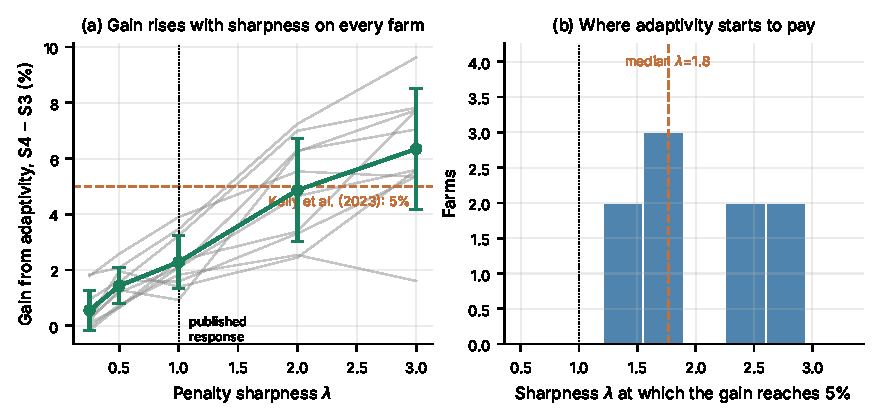
\includegraphics[width=\columnwidth]{../figs/fig6_sharpness_multifarm.pdf}
\caption{(a) Adaptivity gain against penalty sharpness; grey lines are
individual farms, the marked line their mean and standard deviation.
(b) Sharpness at which each farm's gain reaches five percent.}
\label{fig:sharp6}
\end{figure}
